%========================================================================
% Modelo para elaboracao de textos academicos: TCC, dissertacoes e teses
% Elaborado pelo GISIS - Grupo de Imageamento Sismico e Inversao Sismica.
%========================================================================
\chapter{Metodologia}
\label{ch:metodologia}

Este capítulo dedica-se à minuciosa exposição de todas as informações referentes aos experimentos conduzidos para a avaliação meticulosa da precisão e do desempenho dos métodos de resolução da equação eikonal. Inicialmente, empreende-se uma análise comparativa que abrange tanto a precisão quanto o desempenho, abordando a solução numérica em modelos de propriedades simples e complexas. O escopo dessa comparação visa investigar a precisão em diferentes contextos, nomeadamente em um modelo homogêneo, em um modelo de duas camadas e em um modelo complexo amplamente empregado em análises sísmicas.

Os resultados concernentes ao desempenho são derivados de uma plataforma computacional singular, equipada com um processador Intel i7-12700 que dispõe de 20 núcleos, e uma placa gráfica NVIDIA GeForce RTX 3060 com uma capacidade de armazenamento de 12 GB. Destaca-se que os experimentos foram executados no ambiente do sistema operacional Windows 11, com a virtualização da distribuição Linux Ubuntu por meio do \textit{Windows Subsystem for Linux} (WSL). Ao detalhar cada faceta desses experimentos, busca-se oferecer uma compreensão abrangente e fundamentada acerca da eficácia e da aplicabilidade dos métodos de resolução da equação eikonal em levantamentos sísmicos, considerando diferentes cenários e características dos modelos utilizados.

%Todas as informações dos experimentos realizados para verificar a precisão e a performance dos métodos de resolução da equação eikonal estão descritas neste capítulo. Começando pela comparação de precisão e performance utilizando modelos de propriedades simples e complexos, para averiguar a precisão em um modelo homogêneo, em um modelo de duas camadas e em um modelo complexo amplamente utilizado em análises sísmicas. Os resultados de performance são gerados no mesmo computador tendo um processador Intel i7-12700 com 20 núcleos e uma placa gráfica NVIDIA GeForce RTX 3060 com 12 GB de armazenamento. O sistema operacional Windows 11 é utilizado com a virtualização da distribuição linux Ubuntu via WSL.  

\section{Aplicação em modelo homogêneo}

No decorrer deste estudo, optou-se por empregar um modelo homogêneo caracterizado por uma velocidade constante de 2000 m/s. Este modelo, que abrange dimensões espaciais de 200 $\times$ 200 $\times$ 200 metros, adota um parâmetro de discretização de 1 m, resultando em um total de 201 amostras em cada uma das direções $x$, $y$ e $z$. Destaca-se que a posição da fonte sísmica é centralizada no modelo, conferindo-lhe um caráter representativo e simétrico. A determinação do tempo analítico seguiu uma abordagem que envolveu o cálculo a partir da distância entre a fonte e cada ponto da malha, dividida pela velocidade do modelo. Dessa forma, cada ponto na malha foi associado a um tempo analítico correspondente, estabelecendo uma base para comparações posteriores. Cada método foi submetido a uma avaliação rigorosa em termos de eficiência computacional. Os tempos de execução foram registrados e comparados, destacando as nuances de desempenho entre os métodos. Este enfoque permite uma compreensão aprofundada não apenas da precisão, mas também da eficiência computacional de cada abordagem.

Dentre as diferentes formulações exploradas, merecem especial atenção aquelas propostas por \citeonline{podvin1991finite}, \citeonline{jeong2008fast} e \citeonline{noble2014accurate}. Além disso, como uma extensão valiosa deste estudo, o operador de maior precisão do \textit{Fast Iterative Mehod}, conforme delineado no trabalho de \citeonline{cai2023improved}, foi submetido ao teste com os demais formulações estudadas. Vale ressaltar que o código correspondente a esse operador foi gentilmente disponibilizado pelo autor, especificamente configurado para atender a um teste analítico no formato específico em questão. Na seção destinada à apresentação dos resultados, adota-se a prática de \citeonline{cai2023improved}, expondo apenas a média e o máximo erro. Essa abordagem se alinha não apenas com a acurácia ou performance, mas também com a consistência metodológica, contribuindo para uma compreensão mais clara e concisa dos resultados obtidos neste estudo. 

%Um modelo homogêneo foi aplicado com velocidade constante de 2000 m/s. O modelo tem 200 $\times$ 200 $\times$ 200 metros, com parâmetro de discretização de 1 m, totalizando 201 amostras em cada direção $x$, $y$ e $z$. A posição da fonte se encontra no centro do modelo. O tempo analítico é calculado a partir da distância da fonte a cada ponto da malha dividido pela velocidade do modelo. O erro é computado a partir da diferença entre o tempo numérico e o tempo analítico. As formulações de \citeonline{podvin1991finite}, \citeonline{jeong2008fast} e \citeonline{noble2014accurate} são analisadas. Como caso adicional, o operador mais preciso desenvolvido no trabalho de \citeonline{cai2023improved} é testado, pois o código foi fornecido pelo autor exatamente com um teste analítico nesse formado em questão. Na seção de resultados, somente a média e o máximo erro são mostrados assim como no trabalho de \citeonline{cai2023improved}. 

\section{Aplicação em modelo de refração}

No âmbito de um experimento com elevada relevância, cujos resultados foram submetidos à apreciação do Simpósio Brasileiro de Geofísica \cite{alves2022refraction}, será minuciosamente explorada uma comparação numérica entre as distintas formulações objeto de estudo. Este enfoque visa não apenas elucidar a precisão inerente ao cálculo de ondas refratadas, mas também analisar o comportamento desses métodos quando submetidos ao princípio da reciprocidade. O exemplo esquemático delineia uma configuração específica, na qual uma fonte é estrategicamente posicionada na superfície e no centro do modelo de velocidade. Concomitantemente, um arranjo circular de receptores, espaçados regularmente a intervalos de 50 metros, é distribuído a uma distância de 10 km da fonte. O modelo de velocidades adotado neste cenário particular apresenta apenas uma interface, caracterizada por propriedades de 1500 e 2000 m/s para cada camada. A representação visual dessa configuração experimental, evidenciada na Figura \ref{fig:configurationNumericalComparison}, inclui não apenas a disposição espacial da fonte e dos receptores, mas também um perfil detalhado do modelo de velocidades, bem como cortes do modelo com isócronas de tempo projetadas. No intuito de avaliar a precisão intrínseca dos métodos em questão, foram construídos três modelos de velocidade com distintos espaçamentos: 25, 50 e 100 metros. As dimensões e amostras destes modelos variam proporcionalmente à discretização adotada, sendo ($z$, $x$, $y$) = (12, 221, 221) amostras para o modelo de 100 m, (23, 441, 441) amostras para o modelo de 50 m e (45, 881, 881) amostras para o modelo de 25 m. Além dessa abordagem centrada na precisão das formulações, foi conduzido um estudo de reciprocidade, consistindo na inversão das posições da fonte e dos receptores. Essa análise em larga escala permitiu a observação de efeitos de inicialização em pontos situados fora da malha, contribuindo para uma compreensão mais abrangente do desempenho dos algoritmos estudados. Registrou-se, também, o tempo de execução do problema para 1257 tiros, proporcionando uma métrica temporal significativa para avaliar a eficiência dos métodos em questão. Este estudo compreensivo busca fornecer características valiosas sobre a aplicabilidade e desempenho dos métodos estudados em larga escala.


%Como parte de um experimento apresentado ao Simpósio Brasileiro de Geofísica \cite{alves2022refraction}, uma comparação numérica entre os métodos estudados será abordada, agora demonstrando a precisão no cálculo de ondas refratadas e o comportamento utilizando o princípio da reciprocidade. O exemplo esquemático aloca uma fonte na superfície do centro do modelo de velocidade e um arranjo circular de receptores espaçados regularmente de 50 metros com distância de 10 km da fonte. O modelo de velocidades empregado contém somente uma interface com propriedades de 1500 e 2000 m/s para cada camada. A figura \ref{fig:configurationNumericalComparison} mostra a configuração do experimento, o modelo de velocidades detalhado em forma de perfil e cortes do modelo com as isócronas de tempo projetadas. Para verificar a precisão dos métodos, foram construídos três modelos de velocidade com espaçamentos de 25, 50 e 100 metros. As amostras dos modelos construídos variam com a discretização do modelo sendo ($z$, $x$, $y$) = (12, 221, 221) amostras para o modelo de 100 m, (23, 441, 441) amostras para o modelo de 50 m e (45, 881, 881) amostras para o modelo de 25 m. Um estudo de reciprocidade, invertendo a posição da fonte com os receptores, foi efetuado para averiguar o funcionamento do algoritmo em larga escala. Assim, efeitos de inicialização em pontos fora da malha podem ser notados e o tempo de execução do problema para 1257 tiros pode ser registrado.

\begin{figure}[H]
	\centering
	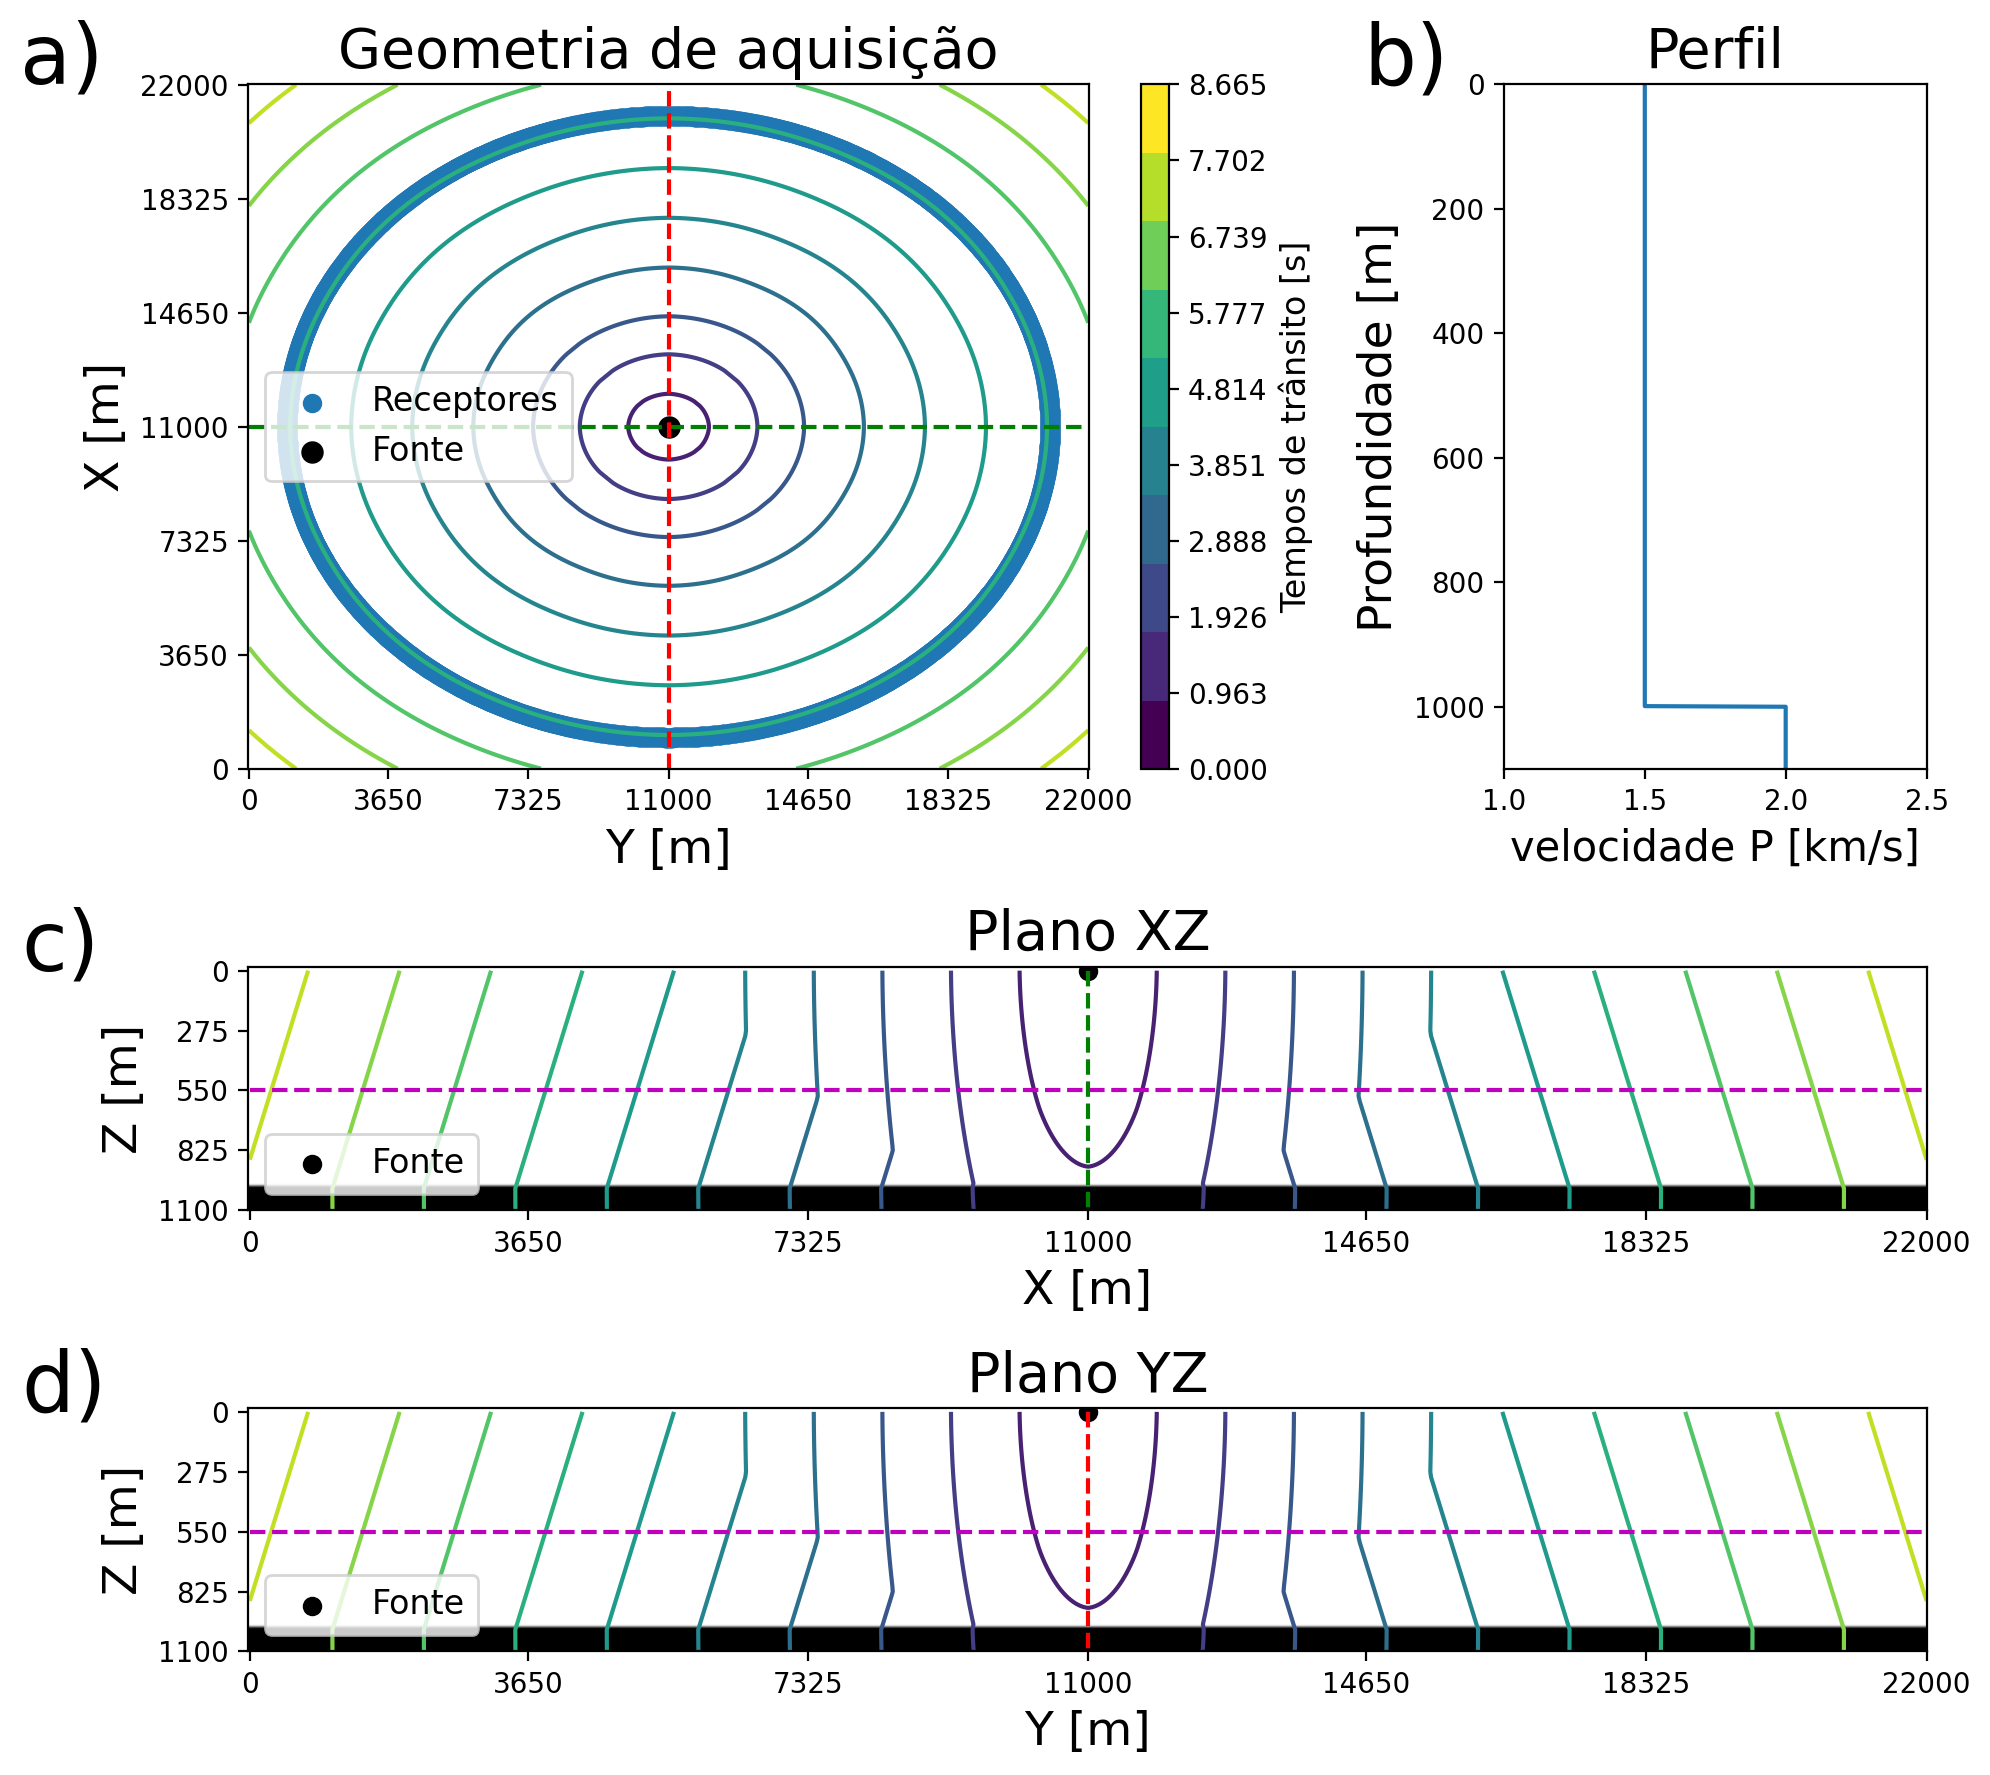
\includegraphics[width = 11cm, height = 10.5cm]{Imgs/RevisaoBibliografica/modelGeometry.png}
	\caption{Modelo empregado no teste de precisão e performance. (a) Plano XY ilustrando a geometria de aquisição com o arranjo de receptores circulares possuindo somente um tiro central. Isócronas mapeando o comportamento dos tempos de trânsito são mostradas. (b) Perfil de velocidades delimitando a posição da interface. (c) e (d) são as projeções dos cortes em planos XZ e YZ em relação à posição da fonte.}
	\label{fig:configurationNumericalComparison}
\end{figure}

\section{Aplicação em modelo complexo}

Com o propósito de validar os algoritmos em um cenário mais próximo da realidade, as formulações estudadas foram aplicadas no modelo SEG/EAGE \textit{Overthrust}, cuja representação visual é proporcionada pela Figura \ref{fig:overthrust}. Este procedimento visa verificar o comportamento das frentes de onda e os tempos de execução diante de uma simulação caracterizada por elevados contrastes de velocidade. O modelo em questão possui dimensões de ($z$, $x$, $y$) = (4.5, 20, 20) km, adotando um parâmetro de discretização de 25 m, o que resulta em um total de (181, 801, 801) amostras. Na configuração específica desse experimento, foi empregado um esquema de geometria circular contendo três círculos na superfície do modelo, distanciados a 5500, 7500 e 9500 metros do centro, onde a posição da fonte está situada. O espaçamento entre os receptores foi estabelecido em 25 m, totalizando 5662 estações, buscando registrar detalhes precisos dos tempos gerados pelas formulações responsáveis por resolver a equação eikonal. Como resultado desse experimento, janelas de aproximação nos dados evidenciam os detalhes que o modelo de alto contraste projeta nos dados calculados. Outro aspecto analisado refere-se aos tempos de execução das formulações propostas por \citeonline{podvin1991finite}, \citeonline{jeong2008fast} e \citeonline{noble2014accurate}, os quais foram mensurados após o cálculo dos tempos das ondas de primeira chegada. 

%A fim de validar os algoritmos em um modelo realístico, as formulações estudadas foram aplicadas no modelo SEG/EAGE \textit{Overthrust}, ilustrado na Figura \ref{fig:overthrust}, na intenção de verificar o comportamento das frentes de onda e os tempos de execução perante uma simulação com altos contrastes de velocidade. O modelo possui dimensões de  ($z$, $x$, $y$) = (4.5, 20, 20) km e parâmetro de discretização de 25 m, totalizando (181, 801, 801) amostras. O esquema de geometria circular foi utilizado possuindo três círculos na superfície do modelo com afastamentos 5500, 7500 e 9500 metros do centro do modelo, onde a posição da fonte se encontra. O espaçamento entre os receptores é de 25 m, totalizando 5662 estações, para registrar o máximo de detalhes possível dos tempos gerados pelas formulações que resolvem a equação eikonal. Como o resultado desse experimento, as primeiras chegadas são apresentadas de forma geral e janelas de aproximação no dado mostram os detalhes que o modelo de alto contraste projeta nos dados calculados. Outro resultado são os tempos de execução das formulações de \citeonline{podvin1991finite}, \citeonline{jeong2008fast} e \citeonline{noble2014accurate} após o cálculo do tempo das ondas de primeira chegada. 

\begin{figure}[H]
	\centering
	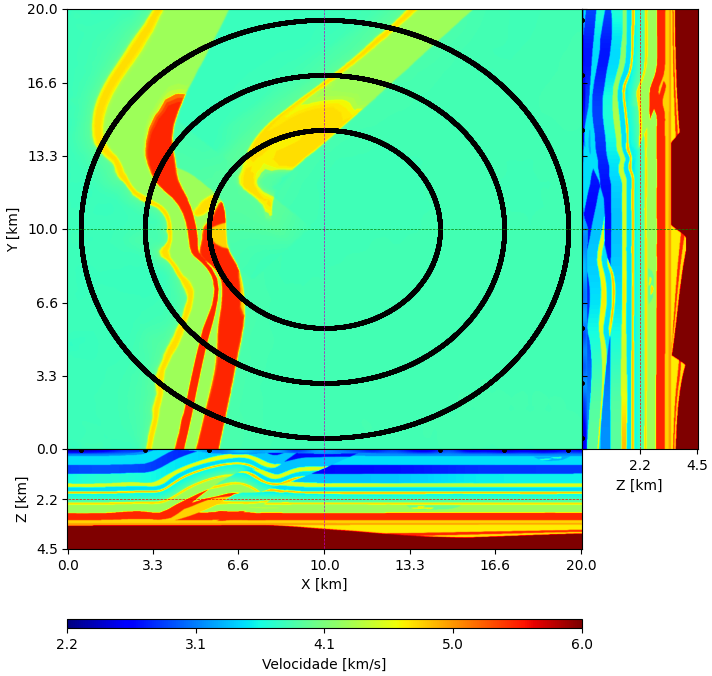
\includegraphics[width = 7.5cm, height = 7.9cm]{Imgs/Metodologia/overthrust.png}
	\caption{Modelo SEG/EAGE \textit{Overthrust} para aplicação dos métodos em altos contrastes de velocidade. A geometria circular é aplicada para verificar o comportamento azimutal dos tempos de trânsito. Em preto são os receptores espaçados em 25 metros totalizando 5662 estações. Uma fonte é a plicada no centro do modelo.}
	\label{fig:overthrust}
\end{figure}







